\documentclass{scrartcl}
\usepackage[paper=a5paper, landscape]{geometry}
\usepackage{hyperref}
\usepackage{fontawesome5}
\usepackage{enumitem}
\usepackage{amsmath, amsfonts, amssymb, mathtools}
\usepackage{tabularx}
\usepackage{pgfplots}

\pgfplotsset{compat=1.18}
\usetikzlibrary{matrix}
\hypersetup{
	colorlinks=true
}
\definecolor{plotGold}{RGB}{184, 134, 61}
\definecolor{bgColor}{RGB}{0, 0, 0}

\newcommand{\code}[1]{\texttt{#1}}
\newcounter{prob}
\newenvironment{problem}[1]{\stepcounter{prob}\paragraph{Problem \theprob} (#1 Points)}{}

\title{\textbf{Overfitting and Underfitting}}
\author{Bhaya, AG\thanks{\faEnvelope[regular] Electronic mail: \href{mailto:contact@angubh.io}{\code{ananya[dot]gb[at]nbu[dot]ac[dot]in}}}}

\begin{document}
	\maketitle
	\pagebreak
	\tableofcontents
	\pagebreak
	
	\section{Introduction}
	\subsection{Overfitting}
	Overfitting is when the model predicts very well on the training data, but poorly on the testing data. Several reasons can lead to overfitting, the most important of which are,
	
	\begin{enumerate}[label*=\Roman*.]
		\item Your model is too complex fo the data (\textit{e.g.} a very tall decision tree or a very deep or wide neural network often overfit).
		\item You have too many features but a small number of training examples.
	\end{enumerate}
	
	\subsection{Underfitting}
	Underfitting is the \textit{inability} of the model to predict well the labels of the data it was trained on. There could be several reasons for underfitting, the most important of which are,
	
	\begin{enumerate}[label*=\Roman*.]
		\item Your model is too simple for the data (\textit{e.g.}, a linear model can often underfit).
		\item The features you engineered are not informative enough.
	\end{enumerate}
	
	The \textbf{solution} to the problem of underfitting is to try a more complex model or to engineer features wiht higher predictive power.
	
	\subsubsection*{Overfitting and underfitting glimpse}
	\begin{table}[ht]
		\centering
		\begin{tabularx}{0.7\textwidth}{|X|X|X|}
			\hline
			& \textbf{Small training error} & \textbf{Large training error}\\ 
			\hline
			\textbf{Small test error} & Generalized & Very unlikely\\ \hline
			\textbf{Large test error} & Overfitting & Underfitting\\ \hline
		\end{tabularx}
	\end{table}
	
	\pagebreak
	
	\begin{problem}{2}
		You trained a regressor model with fixed model complexity, which gives very high accuracy on the training data but much lower accuracy on the validation data. Which of teh following statements may be true? (\textit{Select all that apply}.)
		
		\begin{enumerate}[label*=\Roman*.]
			\item This is an instance of overfitting.
			\item This is an instance of underfitting.
			\item The training and testing examples are sampled from different distributions.
		\end{enumerate}
	\end{problem}
	
	\subparagraph{Sol.} Options (I) and (III) are correct.
	
	\begin{problem}{2}
		``\textit{A regressor with fixed model complexity trained on a smaller dataset is less likely to verfit compared to one trained on a larger dataset.}" Is the statement correct? Justify.
	\end{problem}
	
	\subparagraph{Sol.} The given statement is not correct. The regressor trained on a smaller dataset, is more likly to overfit. Since the dataset is smaller, the model might overfit the noise, leading to inaccuracies.
	
	\begin{problem}{2}
		``\textit{If there is no noise, then there is no overfitting.}" Is the statement correct? Justify.
	\end{problem}
	
	\subparagraph{Sol.} The given statement is not correct. For the training data, one might have \((x,y)\) pairs, which completely satisfy the regressor function \(y=f(x)\). So there will be almost zero training error. But the test points might lie outside the polynomial function (since the test points are not known). Hence, the wrong choice of the polynomial degree can result in overfitting.
	
	\begin{problem}{2}
		Which of the following statements is true?
		
		\begin{enumerate}[label*=\Roman*.]
			\item If there is no noise, then there is no overfitting.
			\item Overfitting may improve the generalization ability of a model.
			\item Generalization error is monotone with respect to the capacity or complexity of a model.
			\item More training data may help preventing overfitting.
		\end{enumerate}
	\end{problem}
	
	\subparagraph{Sol.}
	
	Option (IV) is correct.
	
	\begin{problem}{4}
		Suppose we predict target variable \(y\) using 8 models with different degree of polynomial features (degrees 0 through 7). Which of the following plots display the trainign and validation errors of these models? Assume that we plot the degree of polynomial features on the x-axis, mean squared error loss on the y-axis, and the plots share y-axis limits.
		\begin{figure}[ht]
			\centering
			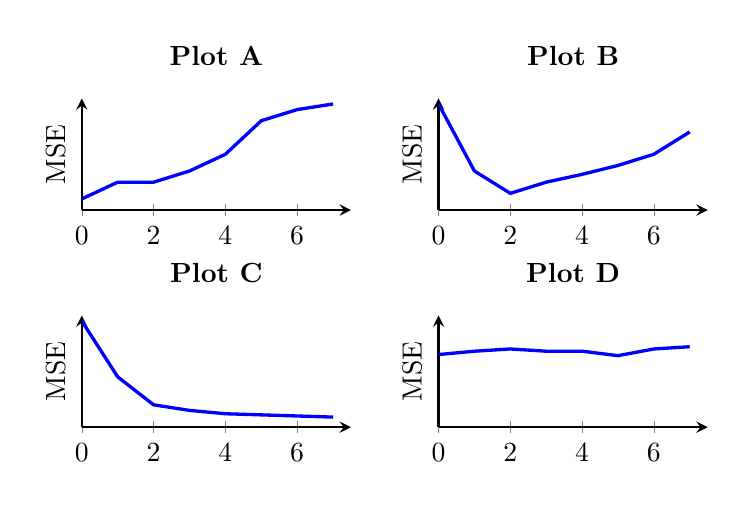
\begin{tikzpicture}
			\pgfplotsset{
				standard/.style={
					width=5cm, height=3cm,
					axis lines=left,
					title style={at={(0.5,1.05)}, anchor=south, font=\bfseries},
					xlabel={}, ylabel={},
					xmin=0, xmax=7.5,
					ymin=0, ymax=10,
					xtick={0,2,4,6},
					ytick=\empty,
					% Black and white styling
					axis line style={black, thick},
					tick label style={black, font=\sffamily},
					% Plot line and marker style
					no markers,
					mark=*,
					mark size=2.5pt,
					mark options={fill=black, draw=black},
					draw=black,
					line width=1.2pt
				}
			}
			
			\matrix[column sep=15pt] {
				% Plot A
				\begin{axis}[standard, title={Plot A}, ylabel={MSE}, ylabel style={black}]
					\addplot coordinates {(0,1) (1,2.5) (2,2.5) (3,3.5) (4,5) (5,8) (6,9) (7,9.5)};
				\end{axis} 
				&
				% Plot B
				\begin{axis}[standard, title={Plot B}, ylabel={MSE}]
					\addplot coordinates {(0,9.5) (1,3.5) (2,1.5) (3,2.5) (4,3.2) (5,4) (6,5) (7,7)};
				\end{axis} 
				\\
				% Plot C
				\begin{axis}[standard, title={Plot C}, ylabel={MSE}]
					\addplot coordinates {(0,9.5) (1,4.5) (2,2) (3,1.5) (4,1.2) (5,1.1) (6,1) (7,0.9)};
				\end{axis} 
				&
				% Plot D
				\begin{axis}[standard, title={Plot D}, ylabel={MSE}]
					\addplot coordinates {(0,6.5) (1,6.8) (2,7) (3,6.8) (4,6.8) (5,6.4) (6,7) (7,7.2)};
				\end{axis} \\
			};
		\end{tikzpicture}
		\end{figure}
		
		From the graphs, identify training and validation error plots.
	\end{problem}
	
	\subparagraph{Sol.} Training error is represented by \textbf{Plot C}, and validation error is represented by \textbf{Plot B}.
	
	\pagebreak
	
	\section{Generalization}
	
	Following statements can be generalized.
	
	\begin{enumerate}[label*=(\Alph*)]
		\item If the model has \textbf{low} training set error and \textbf{low} test set error, the model generalizes.
		\item If the model has \textbf{low} training set error and \textbf{high} test set error, the model overfits.
		\item If the model has \textbf{high} training set error and \textbf{high} test set error, the model underfits.
		\item We can fix underfitting by either usign a \textbf{more} complex model or \textbf{adding} features.
		\item We can fix overfitting by either usign a \textbf{less} complex model or \textbf{removing} features.
	\end{enumerate}
	
\end{document}